\documentclass[11pt]{article}
% Shared preamble for the notes in this repository. pdfLaTeX, TeX Live 2024 or later.
\usepackage[a4paper,margin=2.6cm]{geometry}
\usepackage[T1]{fontenc}
\usepackage{lmodern}
\usepackage{microtype}
\usepackage{amsmath,amssymb,amsthm}
\usepackage{graphicx}
\usepackage{booktabs}
\usepackage{enumitem}
\usepackage[dvipsnames]{xcolor}
\usepackage[hidelinks]{hyperref}
\hypersetup{colorlinks=true,linkcolor=MidnightBlue,citecolor=MidnightBlue,urlcolor=MidnightBlue}
\graphicspath{{../../figures/}}
\setlist{itemsep=2pt,topsep=4pt}

\newtheorem{theorem}{Theorem}
\newtheorem{proposition}[theorem]{Proposition}
\newtheorem{corollary}[theorem]{Corollary}
\newtheorem{conjecture}[theorem]{Conjecture}
\theoremstyle{definition}
\newtheorem{definition}[theorem]{Definition}
% Reusable derivations, numbered note.k; each note sets \notenumber. Indexed in DERIVATIONS.md.
\newcommand{\notenumber}{0}
\newtheorem{derivation}{Derivation}
\renewcommand{\thederivation}{\notenumber.\arabic{derivation}}
\newtheorem{question}{Question}
\theoremstyle{remark}
\newtheorem{remark}[theorem]{Remark}

\newcommand{\Z}{\mathbb{Z}}
\newcommand{\Q}{\mathbb{Q}}
\newcommand{\R}{\mathbb{R}}
\newcommand{\C}{\mathbb{C}}
\newcommand{\HH}{\mathbb{H}}
\newcommand{\SL}{\mathrm{SL}}
\newcommand{\Gal}{\mathrm{Gal}}
\newcommand{\Hom}{\mathrm{Hom}}
\newcommand{\repo}{\href{https://github.com/rmorleysmith/l-functions-and-physics}{\texttt{l-functions-and-physics}}}
\newcommand{\formal}{\href{https://github.com/rmorleysmith/morley-smith-formal}{\texttt{morley-smith-formal}}}
\newcommand{\script}[1]{\href{https://github.com/rmorleysmith/l-functions-and-physics/blob/main/scripts/#1}{\texttt{scripts/#1}}}
% A path inside the Lean repository; it may break after a slash.
\newcommand{\leanpath}[1]{\nolinkurl{#1}}

% Grades used in every status table.
\newcommand{\gradeLean}{\textsc{lean}}      % proved in Lean 4 with Mathlib
\newcommand{\gradeClassical}{\textsc{classical}}  % a published theorem, cited
\newcommand{\gradeComputed}{\textsc{computed}}    % checked numerically by a script in this repository
\newcommand{\gradeConvention}{\textsc{convention}}  % a choice of units or names
\newcommand{\gradeOpen}{\textsc{open}}      % a question, conjecture or working hypothesis
% The legend printed under every status table.
\newcommand{\gradelegend}{\par\nopagebreak\smallskip\noindent\begin{minipage}{\textwidth}\small
\gradeLean: proved in Lean 4 with Mathlib.
\gradeClassical: a published theorem.
\gradeComputed: checked numerically by a script in the repository \repo.
\gradeConvention: a choice of units or names.
\gradeOpen: a question, conjecture or working hypothesis.
\end{minipage}\par\medskip}
% A plain-language physical reading, placed after each derivation.
\newcommand{\physical}{\paragraph{In physical terms.}}

\renewcommand{\notenumber}{12}

\title{Lattice metrics and the cosmological-term functional\\ of gravity from entropy}
\author{Richard Morley-Smith}
\date{Note 12 \quad November 2026}

\begin{document}
\maketitle

\begin{abstract}
\noindent
The theory of gravity from entropy of Bianconi has an emergent cosmological term $\Lambda_{\mathcal G}$ proportional to $\mathrm{Tr}(\mathcal G-I-\ln\mathcal G)$, where $\mathcal G = [\tilde{\mathbf G}\tilde g^{-1}]^{-1}$ for the metric $\tilde g$ of spacetime and the metric $\tilde{\mathbf G}$ induced by matter and curvature.
We evaluate this functional on positive definite binary quadratic forms of determinant one, the normalised Gram matrices of plane lattices.
For two such metrics it equals $2\cosh\delta-2$, where $\delta$ is the hyperbolic distance between the corresponding points $z$, $w$ of the upper half-plane.
For a lattice and the same lattice in a new basis, related by $\gamma\in\SL(2,\Z)$ of trace $t$, it is at least the discriminant $t^2-4$, with equality on the axis of $\gamma$; over hyperbolic $\gamma$ its least value is $5$, attained by $\left(\begin{smallmatrix}2&1\\1&1\end{smallmatrix}\right)$.
These statements are proved in Lean, the equality case as the vanishing of an explicit quadratic expression.
Dirichlet's class number formula then expresses the ratio of the length of the closed geodesic of $\gamma$ to $\sqrt{t^2-4}$ as a rational multiple of $L(1,\chi_D)$.
The functional $S$ is twice a Kullback--Leibler divergence, and $\tfrac12k_BT\,S$ is the mean work dissipated when a harmonic trap is switched suddenly from one thermal covariance to another.
\end{abstract}

\section{The functional}

In the theory of gravity from entropy \cite{BianconiGfE, BianconiLambda} the higher-order metric $\tilde g$ of spacetime and a higher-order metric $\tilde{\mathbf G} = \mathbf I+\alpha\tilde M-\beta\tilde R$, induced by the matter fields through $\tilde M$ and by the curvature $\tilde R$, are treated as operators.
The Lagrangian is the geometric quantum relative entropy
\[
  \mathcal L_{\mathrm{GfE}} = -\mathrm{Tr}_F\ln\bigl(\tilde{\mathbf G}\,\tilde g^{-1}\bigr)
\]
(equations (5) and (9) of \cite{BianconiLambda}).
Here $\mathrm{Tr}_F$ is the flattened trace of \cite{BianconiGfE}, taken over the direct sum of the 0-, 1- and 2-form components of the metrics of a four-dimensional Lorentzian spacetime.
The constraint $\tilde\Theta = \tilde{\mathbf G}\,\tilde g^{-1}$ is imposed with Lagrange multipliers $\tilde{\mathcal G}$, the G-field, which is related to it by $\tilde{\mathcal G} = \tilde\Theta^{-1}$, the stationarity condition of the constrained Lagrangian in $\tilde\Theta$.
The Lagrangian then contains the emergent cosmological term
\[
  \Lambda_{\mathcal G} = \frac{1}{6\beta}\,\mathrm{Tr}_F\bigl[\tilde{\mathcal G}-\tilde I-\ln\tilde{\mathcal G}\bigr]
\]
(equations (14) to (20) of \cite{BianconiLambda}), which is non-negative and which the theory interprets as an internal energy density (\cite{BianconiLambda}, section~1, after \cite{BianconiThermo}).
The function $x\mapsto x-1-\ln x$, applied to the eigenvalues of $\tilde{\mathcal G}$, is non-negative and vanishes only at $x=1$.

For positive definite $n\times n$ matrices $A$ and $B$ we write the corresponding expression as
\[
  S(A,B) = \mathrm{tr}\bigl(G-1-\log G\bigr) = \mathrm{tr}\,G-n-\log\det G,\qquad G = AB^{-1},
\]
with $A$ in the place of $\tilde g$ and $B$ in the place of $\tilde{\mathbf G}$, so that $G$ corresponds to $\tilde{\mathcal G}$ and $S$ to $6\beta\Lambda_{\mathcal G}$.
The Lagrangian itself becomes $\log\det G$; in particular it is zero on the lattice metrics of section~\ref{sec:lattice}, which all have determinant one.
$S$ is the log-determinant divergence of $A$ from $B$, and it is twice the Kullback--Leibler divergence $\mathrm{KL}\bigl(N(0,A)\,\|\,N(0,B)\bigr)$ of the centred Gaussian distributions: the logarithm of the ratio of the two densities is $\tfrac12\log(\det B/\det A)-\tfrac12x^{\mathsf T}A^{-1}x+\tfrac12x^{\mathsf T}B^{-1}x$, and the mean of $x^{\mathsf T}Cx$ under $N(0,A)$ is $\mathrm{tr}(CA)$.

\physical
A classical particle in a harmonic trap with stiffness matrix $K$ at temperature $T$ has position covariance $k_BT\,K^{-1}$.
Let the particle be in equilibrium with covariance $A$, and switch the stiffness instantly from $k_BT\,A^{-1}$ to $k_BT\,B^{-1}$.
The work done on the particle is $W = \tfrac12x^{\mathsf T}(K_B-K_A)x$, with mean $\tfrac12k_BT(\mathrm{tr}\,G-n)$, and the free energy changes by $\Delta F = \tfrac12k_BT\log\det G$.
So the mean dissipated work $\langle W\rangle-\Delta F$ is $\tfrac12k_BT\,S(A,B)$, that is, $k_BT$ times the Kullback--Leibler divergence.

\section{Lattice metrics}\label{sec:lattice}

A point $z = x+iy$ of the upper half-plane gives the lattice $\Z+\Z z$ with the oriented basis $(z,1)$; every lattice in $\C$ with an oriented basis is $c(\Z+\Z z)$ for a unique such $z$ and some $c\in\C^\times$, and we call $z$ the shape of the based lattice.
The Gram matrix of the basis, divided by the covolume $y$, is
\[
  M(z) = \frac1y\begin{pmatrix}x^2+y^2 & x\\ x & 1\end{pmatrix},\qquad \det M(z) = 1 .
\]
Every positive definite binary quadratic form of determinant one is $M(z)$ for exactly one $z$: the form $\left(\begin{smallmatrix}A&B\\B&C\end{smallmatrix}\right)$ with $AC-B^2=1$ is $M\bigl((B+i)/C\bigr)$.
For $\gamma = \left(\begin{smallmatrix}a&b\\c&d\end{smallmatrix}\right)\in\SL(2,\Z)$ the basis $(az+b,\,cz+d)$ of the same lattice has normalised Gram matrix $\gamma M(z)\gamma^{\mathsf T} = M(\gamma z)$.
The square lattice has shape $z=i$ and the hexagonal lattice $z=\rho=e^{2\pi i/3}$ (notes~01 and~02).

\begin{derivation}[the divergence is a function of hyperbolic distance]\label{d:distance}
For $z$, $w$ in the upper half-plane let $G = M(z)M(w)^{-1}$ and let $\delta = \delta(z,w)$ be the hyperbolic distance.
Then $\det G = 1$ and $\mathrm{tr}\,G = 2\cosh\delta$, so the eigenvalues of $G$ are $e^{\delta}$ and $e^{-\delta}$, and
\[
  \boxed{\;S\bigl(M(z),M(w)\bigr) = 2\cosh\delta(z,w)-2 = \frac{|z-w|^2}{\mathrm{Im}\,z\,\mathrm{Im}\,w}\;}
\]
\end{derivation}

\noindent
For $w = x'+iy'$ the trace is $(|z|^2-2xx'+|w|^2)/(yy') = 2+|z-w|^2/(yy')$.
The right side is $4u(z,w)$, with $u$ the point-pair invariant of the hyperbolic plane \cite{Iwaniec}; the derivation is classical, and it is proved in Lean in \formal{} (\leanpath{MorleySmithFormal/LatticeMetricDivergence}).
For small $\delta$, $S = \delta^2+\delta^4/12+O(\delta^6)$, and the second-order term $\tfrac12\mathrm{tr}\bigl((M^{-1}dM)^2\bigr) = (dx^2+dy^2)/y^2$ is the hyperbolic metric: the Fisher information metric of the family of Gaussian distributions $N(0,M(z))$.
For metrics whose areas are in the ratio $s$, $\mathrm{tr}(sG) = s\,\mathrm{tr}\,G$ and $\det(sG) = s^2$ give $S(sM(z),M(w)) = 2s\cosh\delta-2-2\log s$, which is convex in $s$ with minimum $2\log\cosh\delta$ at $s = 1/\cosh\delta$.

The bases $(i,1)$ and $(\rho,1)$ of the square and hexagonal lattices are at $S = 2(2/\sqrt3-1) = 0.309\,401\ldots$, and this is the least value of $S(M(i),M(\gamma\rho))$ over $\gamma\in\SL(2,\Z)$.
Indeed $\cosh\delta(i,w) = (|w|^2+1)/(2\,\mathrm{Im}\,w)$ and $\mathrm{Im}\,\gamma\rho = (\sqrt3/2)/(c^2-cd+d^2)$.
If $c^2-cd+d^2 = 1$ then $\gamma\rho = \rho+n$ for an integer $n$, and $\cosh\delta\ge2/\sqrt3$, with equality for $n = 0, 1$; otherwise $c^2-cd+d^2\ge3$, so $\mathrm{Im}\,\gamma\rho\le\sqrt3/6$ and $\cosh\delta\ge13/(4\sqrt3)$.

\physical
A sudden switch between traps with thermal covariances $\sigma^2M(z)$ and $\sigma^2M(w)$ dissipates on average $k_BT(\cosh\delta(z,w)-1)$.
For a small change of shape the mean dissipation is $\tfrac12k_BT\,\delta^2$ to leading order in $\delta$: the hyperbolic metric of the upper half-plane is the Fisher metric of the thermal fluctuations.

\begin{derivation}[a change of basis costs at least the discriminant]\label{d:basis}
For $\gamma = \left(\begin{smallmatrix}a&b\\c&d\end{smallmatrix}\right)\in\SL(2,\Z)$ with trace $t = a+d$,
\[
  S\bigl(M(z),M(\gamma z)\bigr) = t^2-4+\frac{\bigl(c(x^2+y^2)+(d-a)x-b\bigr)^2}{y^2}.
\]
So $S\ge t^2-4$, with equality exactly when $c(x^2+y^2)+(d-a)x-b = 0$, which for $|t|>2$ is the axis of $\gamma$.
For $|t|>2$, $S\ge5$, and $\left(\begin{smallmatrix}2&1\\1&1\end{smallmatrix}\right)$ attains $5$ at $z=i$.
\end{derivation}

\noindent
This is Derivation~\ref{d:distance} combined with the displacement formula of note~05 for $\cosh\delta(z,\gamma z)$, and the bound $5$ is the classical fact that the shortest closed geodesic of the modular surface has length $4\log\varphi$.
The formula, the bound $t^2-4$ with its equality case (as the vanishing of $c(x^2+y^2)+(d-a)x-b$), and the value $5$ are proved in Lean in the same place.
For $\left(\begin{smallmatrix}0&-1\\1&0\end{smallmatrix}\right)$, of trace $0$, the divergence is $(x^2+y^2+1)^2/y^2-4$, which vanishes only at its fixed point $i$; for $\left(\begin{smallmatrix}1&1\\0&1\end{smallmatrix}\right)$ it is $1/y^2$.

\physical
Two descriptions of one lattice, in bases related by a hyperbolic $\gamma$, are separated by a divergence of at least $t^2-4$ for every shape; a sudden switch of a trap from one description to the other dissipates on average at least $\tfrac12k_BT(t^2-4)$.
The least value over all hyperbolic changes of basis is $5$, the discriminant of $\Q(\sqrt5)$, and it is reached on the axis of $\left(\begin{smallmatrix}2&1\\1&1\end{smallmatrix}\right)$, the semicircle from $-1/\varphi$ to $\varphi$ that projects to the shortest closed geodesic of the modular surface (Figure~\ref{fig:divergence}, left).

\begin{figure}[ht]
  \centering
  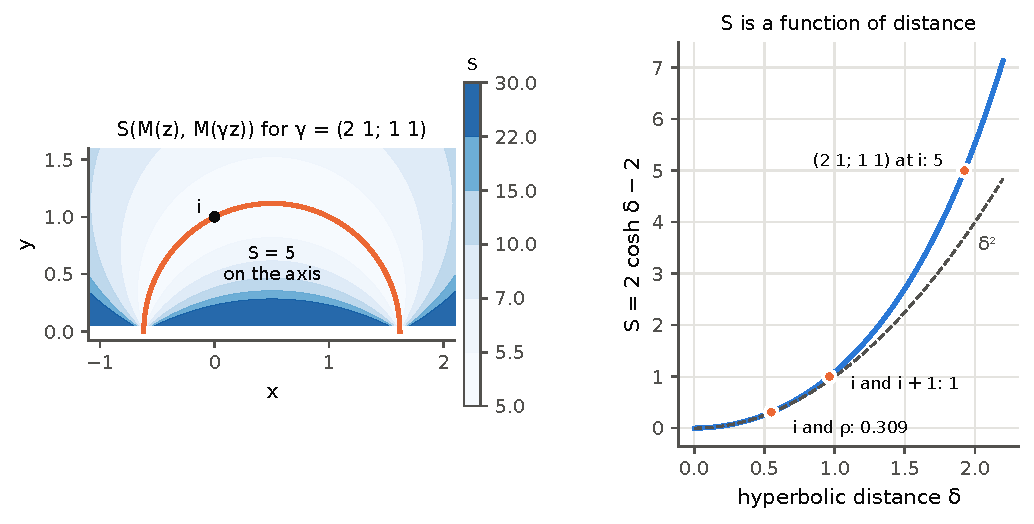
\includegraphics[width=0.98\textwidth]{divergence-lattices}
  \caption{Left: $S(M(z),M(\gamma z))$ for $\gamma = \left(\begin{smallmatrix}2&1\\1&1\end{smallmatrix}\right)$; it equals 5 on the axis, the semicircle from $-1/\varphi$ to $\varphi$ through $i$. Right: $S = 2\cosh\delta-2$ against the hyperbolic distance, with three examples and the quadratic term $\delta^2$.}
  \label{fig:divergence}
\end{figure}

\section{The minimum, the geodesic and an $L$-value}

Let $\gamma$ be hyperbolic with trace $t>2$, and put $\varepsilon_t = \tfrac12\bigl(t+\sqrt{t^2-4}\bigr)$.
Its translation length is $\ell = 2\,\mathrm{arccosh}(t/2) = 2\log\varepsilon_t$; for primitive $\gamma$ this is the length of a closed geodesic of the modular surface (note~05).
Let $S_\gamma = \min_z S(M(z),M(\gamma z))$; by Derivation~\ref{d:basis},
\[
  S_\gamma = t^2-4 = 4\sinh^2\tfrac{\ell}{2} = \bigl(\varepsilon_t-\varepsilon_t^{-1}\bigr)^2 .
\]
Write $t^2-4 = Df^2$ with $D$ a fundamental discriminant and $f\ge1$.
Let $\chi_D = (D/\cdot)$ be the Kronecker symbol, $h(D)$ the class number of $\Q(\sqrt D)$, and $\varepsilon_D>1$ its fundamental unit, of norm $1$ or $-1$; then $\varepsilon_t = \varepsilon_D^{\,k}$ for an integer $k\ge1$.

\begin{derivation}[Dirichlet's formula as a relation between length and minimum]\label{d:lvalue}
With this notation,
\[
  \boxed{\;\frac{\ell}{\sqrt{S_\gamma}} = \frac{k}{h(D)\,f}\;L(1,\chi_D)\;}
\]
\end{derivation}

\noindent
This is Dirichlet's class number formula, here in the normalisation $h(D)\log\varepsilon_D = \tfrac12\sqrt D\,L(1,\chi_D)$ with the class number of the field and its fundamental unit \cite{Davenport}, combined with $\log\varepsilon_D = \ell/(2k)$ and $\sqrt D = \sqrt{S_\gamma}/f$.
The script computes $D$, $f$, $\varepsilon_D$, $k$ and $h(D)$ (from the cycles of reduced indefinite forms), and $L(1,\chi_D) = -D^{-1/2}\sum_{a<D}\chi_D(a)\log\sin(\pi a/D)$, and checks the formula for $t = 3,\dots,11$:

\begin{center}
\small
\begin{tabular}{@{}rrrrlrrc@{}}
\toprule
$t$ & $S_\gamma$ & $D$ & $f$ & $\varepsilon_D$ & $k$ & $h(D)$ & $h(D)f/k$\\
\midrule
3 & 5 & 5 & 1 & $\tfrac12(1+\sqrt5)$ & 2 & 1 & $\tfrac12$\\
4 & 12 & 12 & 1 & $2+\sqrt3$ & 1 & 1 & 1\\
5 & 21 & 21 & 1 & $\tfrac12(5+\sqrt{21})$ & 1 & 1 & 1\\
6 & 32 & 8 & 2 & $1+\sqrt2$ & 2 & 1 & 1\\
7 & 45 & 5 & 3 & $\tfrac12(1+\sqrt5)$ & 4 & 1 & $\tfrac34$\\
8 & 60 & 60 & 1 & $4+\sqrt{15}$ & 1 & 2 & 2\\
9 & 77 & 77 & 1 & $\tfrac12(9+\sqrt{77})$ & 1 & 1 & 1\\
10 & 96 & 24 & 2 & $5+2\sqrt6$ & 1 & 1 & 2\\
11 & 117 & 13 & 3 & $\tfrac12(3+\sqrt{13})$ & 2 & 1 & $\tfrac32$\\
\bottomrule
\end{tabular}
\end{center}

\noindent
For $t=3$ it reads $L(1,\chi_5) = 2\log\varphi/\sqrt5$, with $\ell = 4\log\varphi$ and $S_\gamma = 5$.

\physical
For a hyperbolic change of basis, the least mean dissipation $\tfrac12k_BT\,S_\gamma$ and the length $\ell$ of the closed geodesic determine each other through $S_\gamma = 4\sinh^2(\ell/2)$, and $\ell/\sqrt{S_\gamma} = \bigl(k/(h(D)f)\bigr)\,L(1,\chi_D)$.

\section{Scope}

The model consists of two flat metrics of a two-dimensional lattice; the functional of $\Lambda_{\mathcal G}$ is evaluated on them, and nothing is varied.
In the theory the second metric is induced by the matter fields and the curvature; here it is the metric of the same lattice in another basis, or of another lattice.

\section*{Status of the statements}

\begin{center}
\small
\begin{tabular}{@{}p{0.66\textwidth}l@{}}
\toprule
Statement & Grade\\
\midrule
The Lagrangian, the G-field and $\Lambda_{\mathcal G}$ in the theory of gravity from entropy \cite{BianconiGfE, BianconiLambda, BianconiThermo} & \gradePhysics\\
$S$ is twice a Kullback--Leibler divergence; the mean dissipated work in a sudden switch of a harmonic trap (derived above) & \gradeComputed\\
Derivation~\ref{d:distance}: $\det G = 1$, $\mathrm{tr}\,G = 2\cosh\delta$, the eigenvalues, $S = 2\cosh\delta-2$ & \gradeClassical, \gradeLean, \gradeComputed\\
The Fisher metric; metrics of unequal area & \gradeComputed\\
The square and hexagonal bases: $S = 2(2/\sqrt3-1)$, the least value over the orbit of $\rho$ (proved above; checked on the orbit) & \gradeComputed\\
Derivation~\ref{d:basis}: the formula, the bound $t^2-4$ and its equality case, the bound $5$ and its attainment & \gradeClassical, \gradeLean, \gradeComputed\\
Derivation~\ref{d:lvalue}: Dirichlet's class number formula; the table for $t = 3,\dots,11$ & \gradeClassical, \gradeComputed\\
\bottomrule
\end{tabular}
\end{center}
\gradelegend

\noindent
All checks are in \script{lattice\_divergence.py}.

\begin{thebibliography}{9}
\bibitem{BianconiGfE} G.~Bianconi, Gravity from entropy, \emph{Phys. Rev. D} 111 (2025), 066001.
\bibitem{BianconiLambda} G.~Bianconi, $\Lambda$-Gravity from entropy, \emph{Phys. Lett. B} 882 (2026), 141014; arXiv:2610.34496.
\bibitem{BianconiThermo} G.~Bianconi, Thermodynamics of the gravity from entropy theory, \emph{Phys. Rev. D} 114 (2026), 024042; arXiv:2510.22545.
\bibitem{Davenport} H.~Davenport, \emph{Multiplicative Number Theory}, 3rd ed., Springer, 2000.
\bibitem{Iwaniec} H.~Iwaniec, \emph{Spectral Methods of Automorphic Forms}, 2nd ed., American Mathematical Society, 2002.
\end{thebibliography}

\end{document}
